%% \newcommand{\AAA}{\E[\mathbbm{T}_{4,4}] + \frac{1}{3}\E[\mathbbm{T}_{3,4}] + \frac{2}{9}\E[\mathbbm{T}_{2,4}]}
%% \newcommand{\BBB}{\frac{1}{9}\E[\mathbbm{T}_{2,4}] + \frac{1}{6}\E[\mathbbm{T}_{3,4}]}
%% \newcommand{\CCC}{\E[\mathbbm{T}_{4,4}] - \frac{1}{6}\E[\mathbbm{T}_{3,4}] - \frac{1}{9}\E[\mathbbm{T}_{2,4}]}

In the derivation of the normal model it was assumed that $L\T m_3$, $L \T m_4$,
and $L \left( \T \right)^2 m_2$ go to zero as $L\to \infty$. The expectations of
the third and fourth moments thus go to zero and $3\left(L \T
\E[\mathbbm{T}_{2,2}] m_2\right)^2$ as expected for a normal distribution.
Deviations of the population distribution from normality depend on the
distribution of coalescent times as well as the genetic architecture, and they
can be investigated by comparison to the expected moments under normality. Even
though recombination is not included in the model, we can form an idea about how
linkage might impact deviations from normality by looking at line two of
equation \eqref{eq:emoms4}. This line corresponds to the contribution from two
mutations occurring at a locus. The first part indicates that the expected
fourth moment increases with the variance of the pairwise coalescence time. The
second part is much harder to interpret but seems likely also to be positive.
Overall, this agrees with the notion that linkage disequilibrium increases
deviations from normality by reducing the effective number of loci.

When the mutation rate is low, the ratio of the expected fourth moment to that
under normality is
\begin{equation}
  \label{eq:popmom4coal}
  \frac{\E[M_4]}{3\left(L \T \E[\mathbbm{T}_{2,2}] m_2\right)^2} \approx 1 +
  \frac{\kappa}{6 L \T \E[\mathbbm{T}_{2,2}]}\left( \frac{2\E[\mathbbm{T}_{4,4}] +
      \frac{2}{3}\E[\mathbbm{T}_{3,4}] +
      \frac{4}{9}\E[\mathbbm{T}_{2,4}]}{\E[\mathbbm{T}_{2,2}]}\right),
\end{equation}
where $\kappa$ is the kurtosis of the mutational distribution. The expected
excess in $M_4$ is inversely related to the expected sparsity of the trait which
is proportional to $L \T \E[\mathbbm{T}_{2,2}]$. This excess depends on
demography through a factor $Q = \frac{2\E[\mathbbm{T}_{4,4}] +
  \frac{2}{3}\E[\mathbbm{T}_{3,4}] +
  \frac{4}{9}\E[\mathbbm{T}_{2,4}]}{\E[\mathbbm{T}_{2,2}]}$. The extent to which
demography increases or decreases deviations from normality can be investigated
by calculating $Q$ in different models. In a constant-size and panmictic
population $Q$ is equal to one. In a population where lineages are exchangeable,
$\E[\mathbbm{T}_{i,j}]$ can be calculated numerically using expressions from
\citet{Griffiths1998}. Values of $Q$ in an exponentially growing population are
shown in Figure \ref{fig:Qexp}. Holding sparsity and the mutational distribution
constant, a population having undergone exponential growth will have a greater
expected deviation from normality in its trait distribution. However, growth
rates must become greater than the initial coalescent rate for $Q$ to be
increased by more than ten percent.

\begin{figure}
\centering
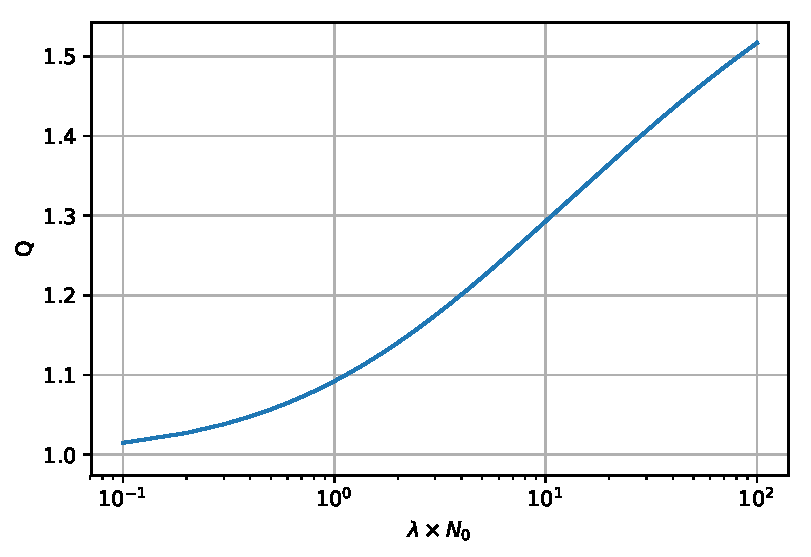
\includegraphics[width=0.65\textwidth]{figures/exp_growth.pdf}
\caption{$Q$ increases as the exponential growth rate increases relative to the current
population size. $\lambda$ is the growth rate and $N_0$ is the initial effective population
size.}
\label{fig:Qexp}
\end{figure}

\begin{figure}
\centering
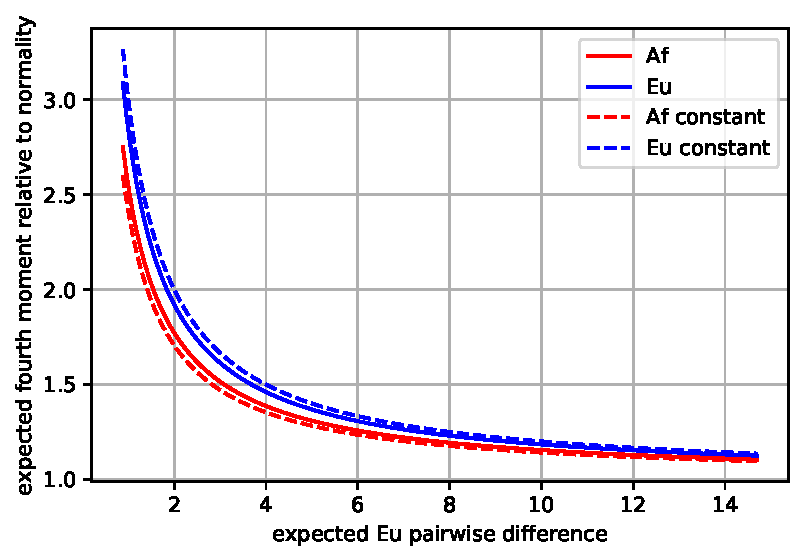
\includegraphics[width=0.65\textwidth]{figures/af_eu_kurt.pdf}
\caption{A comparison between the expected fourth moment under different genetic
architectures in the African and European demographic models fit
by \citet{Tennessen2012}. Genetic architecture is varied by changing the
expected number pairwise differences at sites affecting the trait in the
European model. The mutational kurtosis is set to six. Dashed lines show the
predicted relationship for populations with the same heterozygosity as the
European and African models but with constant size.}
\label{fig:afeucomp}
\end{figure}

As a concrete example we can consider the differences in the expected fourth
moment produced by different demographic histories in different human
populations. In the demographic model fit by \citet{Tennessen2012}, the genetic
European population experiences a bottleneck associated with out-of-Africa and
recent growth while the generic African population experiences a more stable
history also with recent growth. Differences between the two have resulted in a
greater heterozygosity in African populations due to the out-of-Africa
bottleneck \citep{Yu2002}. For a given genetic architecture, the African
population model predicts a smaller deviation from normality than the European
model (Figure \ref{fig:afeucomp}). The expected fourth moment in constant-size
populations with the same heterozygosity as the African and European models is
lower for the African model and higher for the European model. This is because
the African model is dominated by population growth that leads to a $Q$ greater
than one, while the European model is dominated by a bottleneck event that leads
to a $Q$ less than one (Figure \ref{fig:Qland}). However, these difference due
to demography are small and the overall deviations from normality are mostly
driven by sparsity differences.

Another natural way to quantify the deviation of a distribution from normality
is its kurtosis. The kurtosis measures the tendency of a distribution to produce
outliers through the ratio of the fourth central moment to the square of the
variance \citep{Westfall2014}. Since the kurtosis of a trait distribution is
ratio of two random quantities, its expectation is not straightforward to
calculate. A first order approximation is
\begin{equation}
3 + \frac{\kappa \frac{\CCC}{\E[\mathbbm{T}_{2.2}]}} {L \T \E[\mathbbm{T}_{2.2}]
    + \kappa \frac{\BBB}{\E[\mathbbm{T}_{2.2}]}}.
    \label{eq:firstord}
\end{equation}
Although this expression seems to suggest that the expected kurtosis will be
greater than under normality when external branches are longer ($\E[\mathbbm{T}_{4,4}] >
\frac{1}{6}\E[\mathbbm{T}_{3,4}] + \frac{1}{9}\E[\mathbbm{T}_{2,4}]$) and less than under normality
when they are longer ($\E[\mathbbm{T}_{4,4}] < \frac{1}{6}\E[\mathbbm{T}_{3,4}] +
\frac{1}{9}\E[\mathbbm{T}_{2,4}]$), simulations show that the approximation is actually
quite poor (Figure \ref{fig:kurtsim}). The mean kurtosis increases when trait
architecture becomes sparse regardless of whether the population size is
constant or growing. Another feature is that there is substantial variance in
the kurtosis with about a quarter of simulated populations having a kurtosis
less than three even as the mean sharply increases. This high variance is likely
due to a negative correlation between the fourth central moment and the
variance. This, along with the fact that deviations from the infinitesimal model
inflate the fourth moment (equation \eqref{eq:popmom4coal}), leads to a
situation where the kurtosis increases with trait sparsity but the variance is
high across evolutionary realizations.

%%% Local Variables:
%%% TeX-master: "short_report.tex"
%%% End:
